% !TEX root = ../masterthesis.tex
\chapter{Droplet etched gallium arsenide quantum dots}
\label{chapter:quantum-dot}

\section{Fabrication and optical properties}

Quantum dots (\acs{QD}) are nanostructures which confine the motion of electrons and holes in all three spatial dimensions.
Confinement results in discrete energy levels, which is why \acp{QD} are sometimes referred to as \textit{artificial atoms}.
The discussion in this section is based on the PhD thesis of \textcite{huber_gaas_2019}.

Gallium arsenide \acp{QD} investigated within this master's thesis are grown by \ac{MBE} with the self-assembled nanodrill technology described in the work of \textcite{wang_nanoholes_2007}.
As displayed in figure~\ref{fig:droplet-etched-gaas-qds}(a) the \ac{Al} forms droplets on AlGaAs after evaporation.
The \ac{Al} reacts with AlGaAs, which leads into nanoholes etched into te surface.
Under optimal conditions, these nanoholes are highly symmetric as can be seen in figure~\ref{fig:droplet-etched-gaas-qds}(b). 
This results into \ac{QD} with high in-plane symmetry.
The next step is the annealing process in which \ac{GaAs} is deposited to fill the nanoholes.
The \ac{QD} is finalized by capping the layer with AlGaAs acting as top barrier.

Compared to the band gap of the host material Al$_{0.4}$Ga$_{0.6}$As of \SI{1.92}{\electronvolt} at room temperature, the core of the \ac{QD}, \ac{GaAs}, has a band gap of only \SI{1.42}{\electronvolt} at room temperature.
This energy difference between the band gaps and nanosized dimensions of the \ac{QD} are responsible for the 3D confinement and the type-I band alignment depicted in figure~\ref{fig:droplet-etched-gaas-qds}(c).
This thesis focuses on optical transitions between the first energy level in the \ac{CB} and the \ac{VB}, often called the s-shell.
The carriers are the electrons $e^-$ and the holes left behind $h^+$.
These are fermions and therefore only up to two of them can, in accordance with Pauli's exclusion principle, occupy a single energy state.
Electrons and holes are strongly localized inside the \ac{QD} and interact with each other by Coulomb interaction.
This leads to multi-particle complexes with the most fundamental being the \acf{X}, a bound state of an electron and a hole.
A fully occupied s-shell, can be described by the quasiparticle called \acf{XX}.
\begin{figure}[H]
	\centering
	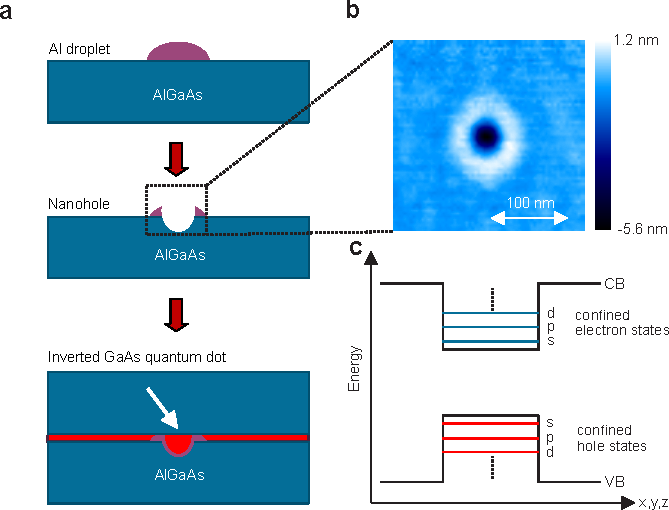
\includegraphics[width=0.8\linewidth]{figures/quantum-dot/droplet-etched-gaas-qds}
	\caption[Droplet etched GaAs quantum dots.]{(a) The growth process of a GaAs quantum dot by \ac{MBE}.\\
	(b) Atomic force microscopy (AFM) image of the nanohole before it is filled with GaAs.\\
    (c) Conduction band (CB) and valence band (VB) of an optically active QD.~\cite{huber_gaas_2019}}
	\label{fig:droplet-etched-gaas-qds}
\end{figure}
In a \ac{QD}, polarization-entangled photon pairs can be generated via a biexciton-exciton cascade~\cite{stevenson_semiconductor_2006}, illustrated in figure~\ref{fig:biexciton-exciton-cascade}.
$\ket{XX}$ forms a full shell, which means that the total angular momentum projection along the quantization axis of the \ac{XX} complex sums up to $M=0$.
After exciting the \ac{QD} into the $\ket{XX}$ state (e.g. by optical pumping) it decays by spontaneous recombination of an electron-hole-pair accompanied by the emission of a single photon into the $\ket{X}$ state.
The two-dipole allowed radiative transitions lead to only two possible $\ket{X}$ states:
\begin{itemize}
	\item $\ket{-1}$ under emission of a right-circularly-polarized photon $\ket{R_{XX}}$ 
	\item $\ket{+1}$ under emission of a left-circularly-polarized photon $\ket{L_{XX}}$ 
\end{itemize}
$\ket{-1}$ and $\ket{+1}$ are degenerate in energy and decay into the groundstate $\ket{G}$ under emission of $\ket{L_X}$ and $\ket{R_X}$, respectively.
The resulting state is then described by
\begin{equation}
\ket{\psi^+}=\frac{1}{\sqrt{2}}\left(\ket{L_{XX}}\ket{R_X}+\ket{R_{XX}\ket{L_X}}\right)
\end{equation}
which is one of the Bell states, representing the maximal entangled states.
\begin{figure}[H]
	\centering
	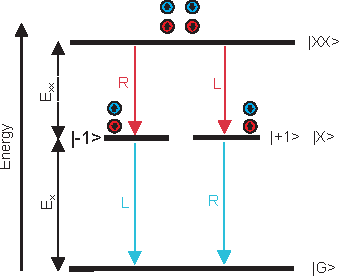
\includegraphics[width=0.5\linewidth]{figures/quantum-dot/biexciton-exciton-cascade}
	\caption{Biexciton-esciton cascade in a QD.~\cite{huber_gaas_2019}}
	\label{fig:biexciton-exciton-cascade}
\end{figure}



\section{Fine structure splitting}
Fine structure splitting (\acs{FSS}) in a \ac{QD} describes the energy splitting between the two possible bright $\ket{X}$ states.
In GaAs it originates from the exchange interaction between electrons and holes.~\cite{bayer_fine_2002}.

In figure~\ref{fig:qd-energy-levels-fss} the $\ket{XX}$ decay path with splitted $\ket{X}$ eigenstates is shown.  $\ket{XX}$ exhibit no splitting as the angular momentum of the electrons and holes add to zero and therefore no exchange interaction occurs.
In figure~\ref{fig:fss-pol} photoluminescence spectra recorded with a linear polarizer are shown.
\begin{figure}[H]
	\centering
	\begin{subfigure}[b]{0.48\textwidth}
		\centering
		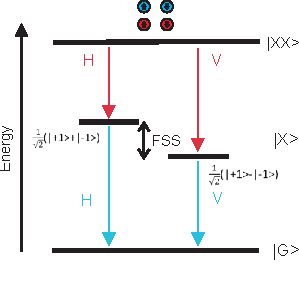
\includegraphics[width=0.95\textwidth]{figures/quantum-dot/QD_EnergyLevels_FSS.pdf}
		\caption{XX decay cascade without X degeneracy because of fine structure splitting.~\cite{huber_gaas_2019}\\}
		\label{fig:qd-energy-levels-fss}
	\end{subfigure}%
	~ % An dieser Stelle kann ein zusätzlicher Zwischenraum eingebunden werden: ~, \quad, \qquad, \hfill usw.
	% Eine leere Zeile erzwingt, dass die zweite Grafik darunter erscheint.
	\begin{subfigure}[b]{0.48\textwidth}
		\centering
		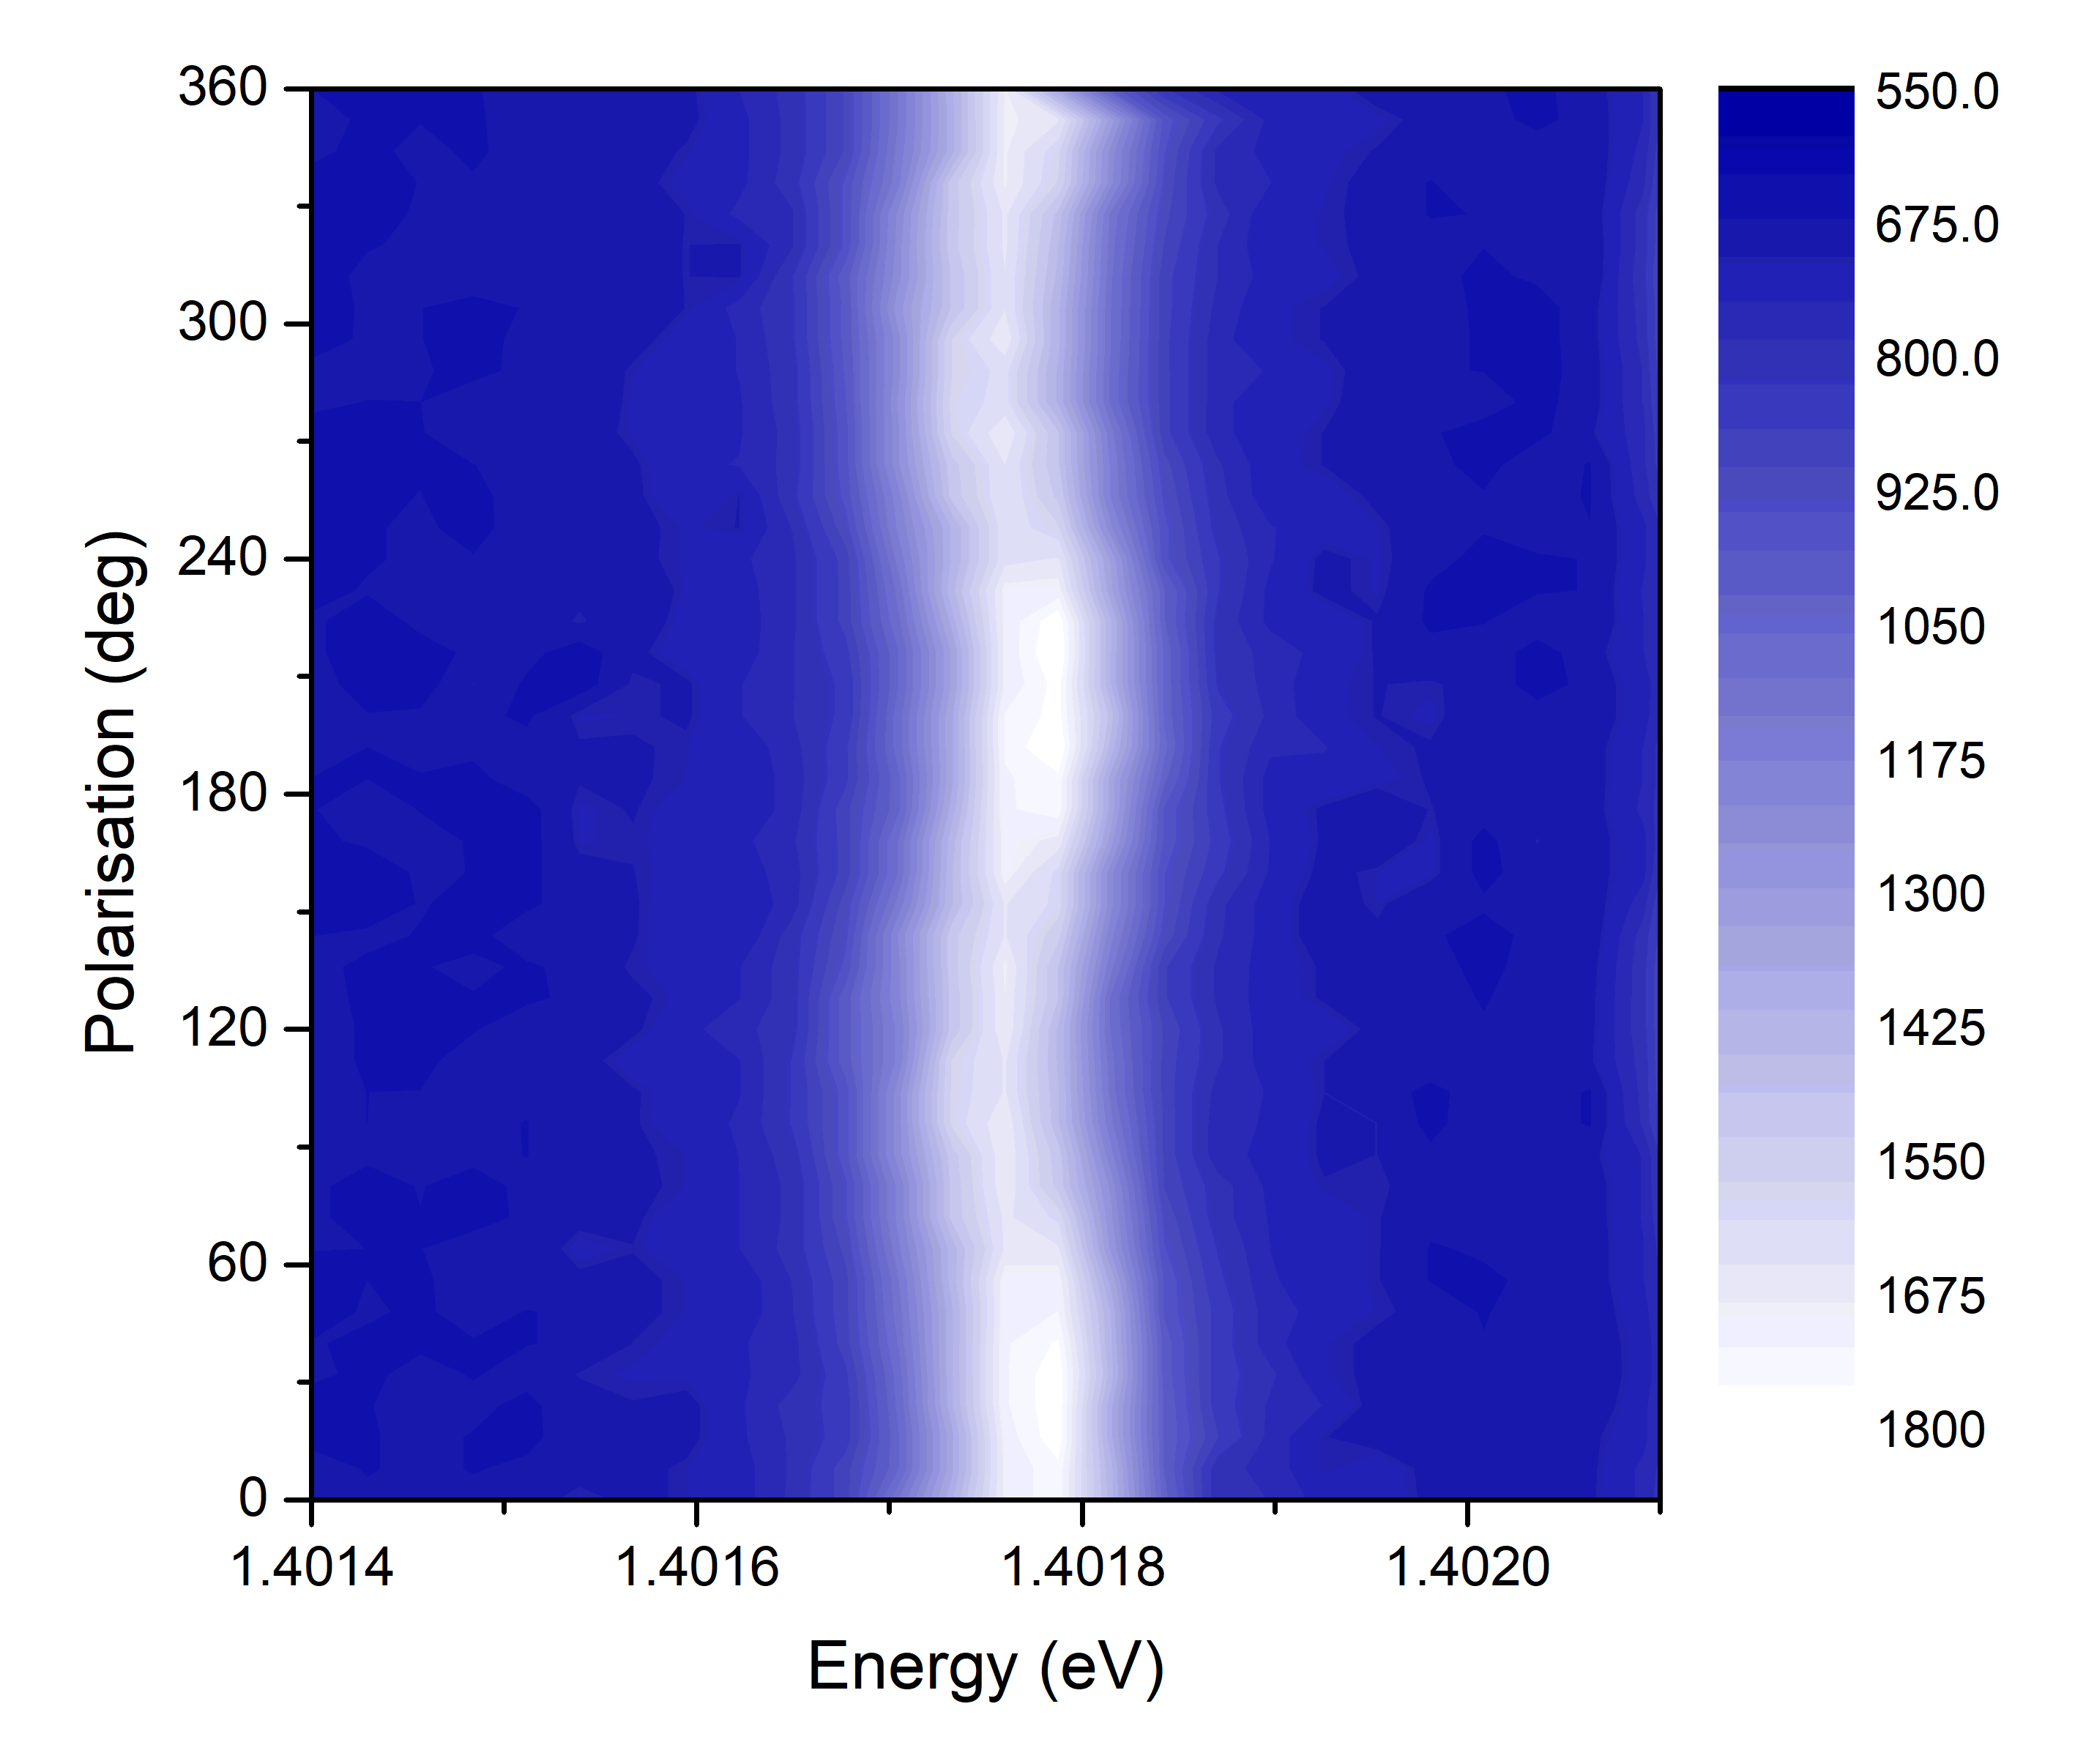
\includegraphics[width=1.05\textwidth]{figures/quantum-dot/FSS_Pol.png}
		\caption{Photoluminescence spectra of X emission of a GaAs Qd plotted for different polarizer angles.
		In the image the effect of the linear polarization of the fine structure components is visible.~\cite{schimpf_towards_2017}}
		\label{fig:fss-pol}
	\end{subfigure}
	\caption{Fine structure splitting in a GaAs quantum dot.}
	\label{fig:fss}
\end{figure}

\section{Zero-phonon line and phonon sideband}
\label{sec:zero-phonon-side-band}
The excitonic emission of \ac{GaAs} \acp{QD} exhibits non-Lorentzian asymmetric broadening. As shown by \textcite{peter_phonon_2004} this side bands can be traced back to a coupling to acoustic phonons.
The discussion of \acp{PSB} is based on \textcite{friedrich_photochemical_1984} and  \textcite{peter_phonon_2004}.

Figure~\ref{fig:line-shape} displays a schematic representation of the \ac{ZPL} and \ac{PSB} absorption spectrum.
The intensity distribution between the two components depends strongly on temperature.
\begin{figure}[H]
	\centering
	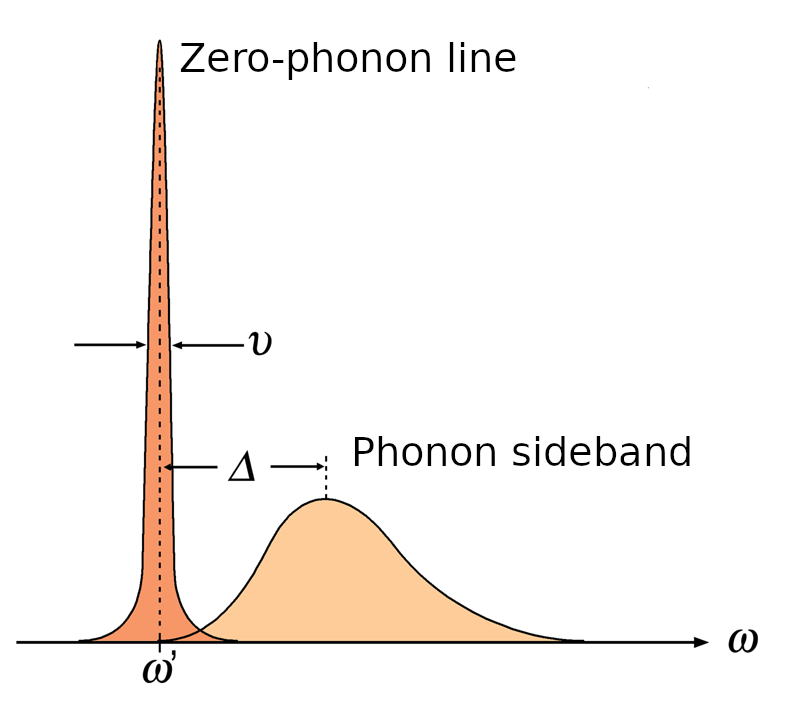
\includegraphics[width=0.6\linewidth]{figures/quantum-dot/Line-shape}
	\caption[Absorption line shape of an electronic excitation.]{Absorption line shape of an electronic excitation.
		The emission is mirrored at $\omega'$.}
	\label{fig:line-shape}
\end{figure}
To determine the frequency gap $\Delta$ the Franc-Condon principles are used.
They state that electronic transition between ground and excited state is much faster than the motion in the lattice.
Hence, there is no motion along the configurational coordinates $q_i$ during the energy transitions as depicted in figure~\ref{fig:phonon-energy-diagram}.
The transitions can be displayed as vertical arrows with the shorter arrow describing the \ac{ZPL} and the longer one describing the \ac{PSB}.
According to the Franc-Condon principles, the more the wave functions of two vibrational energy levels overlap, the likelier is the electronic transition between these two.
In the case of figure~\ref{fig:phonon-energy-diagram} this occurs when the photon energy equals to the energy difference $E_1-E_0$ plus three quanta of vibrational energy $\hbar \Omega_i$.
The emission follows the same principle.
\begin{figure}[H]
	\centering
	\begin{subfigure}[b]{0.48\textwidth}
		\centering
		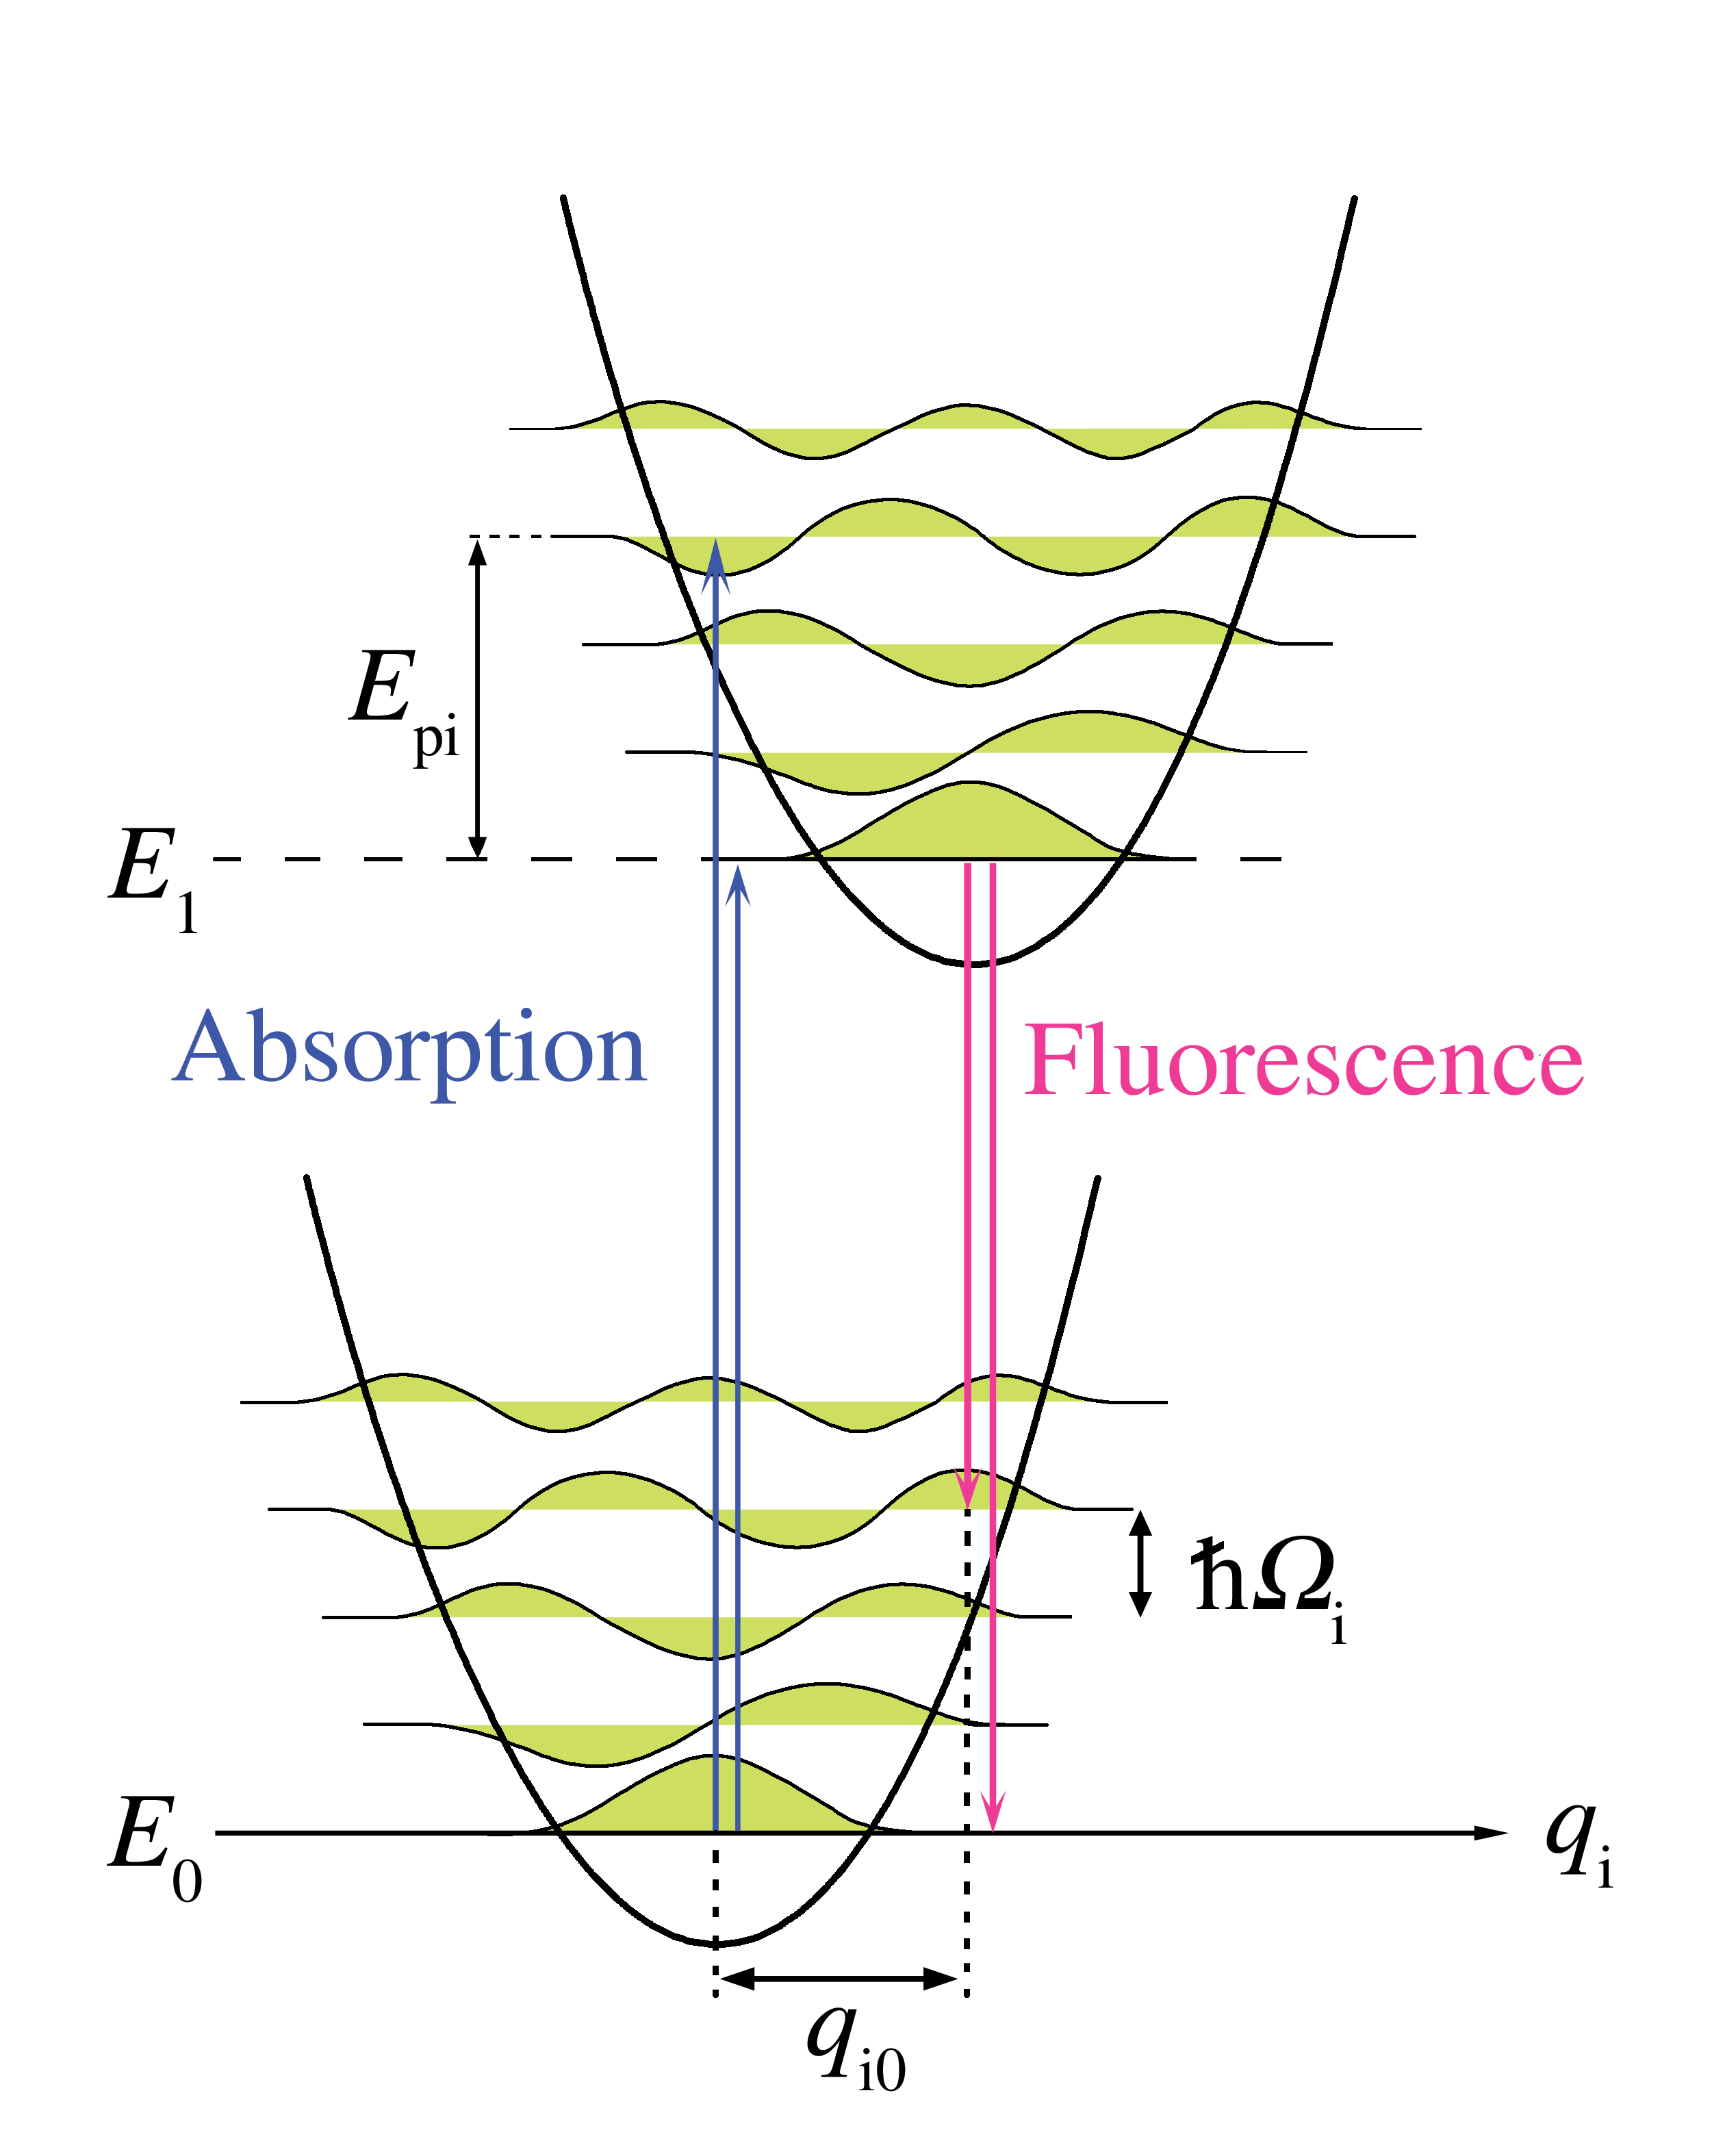
\includegraphics[width=\textwidth]{figures/quantum-dot/Phonon-energy-diagram}
		\caption{Energy spectrum of a two-level electronic system with phonon coupling.
			The arrows describe emission/absorption with and without phonons respectively.}
		\label{fig:phonon-energy-diagram}
	\end{subfigure}%
	~ % An dieser Stelle kann ein zusätzlicher Zwischenraum eingebunden werden: ~, \quad, \qquad, \hfill usw.
	% Eine leere Zeile erzwingt, dass die zweite Grafik darunter erscheint.
	\begin{subfigure}[b]{0.48\textwidth}
		\centering
		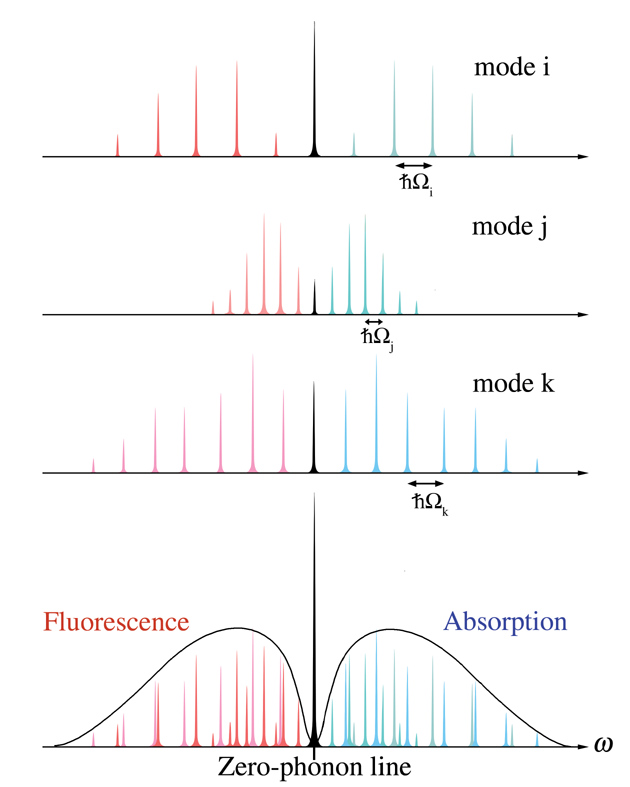
\includegraphics[width=\textwidth]{figures/quantum-dot/Lattice-modes}
		\caption{Three lattice normal modes $(i, j, k)$ and the resulting emission/absorption spectrum.\\}
		\label{fig:lattice-modes}
	\end{subfigure}
	\caption{Zero-phonon line and phonon sideband.~\cite{noauthor_zero-phonon_nodate}}
	\label{fig:zero-phonon-line-phonon-side-band}
\end{figure}
Figure~\ref{fig:phonon-energy-diagram} and \ref{fig:lattice-modes} implicitly assume approximations in addition to the Franck-Condon principles.
The lattice vibrational mode has to be well described by a quantum harmonic oscillator.
Additionally, it is assumed that only the lowest lattice vibration is excited and that the harmonic oscillator potentials are equal in both states.
These preconditions are visible in the equally parabolic shaped potential wells and equally spaced phonon energy levels in figure~\ref{fig:phonon-energy-diagram}.

The zero-phonon line is stronger than the phonon side band because of the superpositon of the lattice modes.
Each lattice mode $m$ leads to a different energy difference $\hbar \Omega_m$ between phonons.
That is why the transitions with phonons result in a energy distribution and the zero-phonon transition add at the electronic origin $E_1 - E_0$ as can be seen in figure~\ref{fig:lattice-modes}b.

The theoretical limit of the spectral range of the zero-phonon line for a GaAs quantum dot can be calculated with the time-energy uncertainty relation
\begin{equation}
\Delta E \cdot \Delta t = \frac{h}{2 \pi}
\end{equation}
This gives for typical lifetime of a GaAs quantum dot of $\Delta t = \SI{250}{\pico \second}$
\begin{equation}
\Delta E = \SI{2.64}{\micro \electronvolt}.
\end{equation}
The frequency uncertainty can be obtained through
\begin{equation}
\label{eq:planck-einstein}
\Delta \nu = \frac{\Delta E}{h}.
\end{equation}
The wavelength $\lambda$ relates to $\nu$ with the Planck-Einstein relation 
\begin{equation}
\lambda(\nu) = \frac{c}{\nu}
\end{equation}
and the wavelength uncertainty $\Delta \lambda$ can be approximated with a Taylor series around $\nu_0$
\begin{align}
\Delta \lambda = - \lambda'(\nu_0)\cdot \Delta \nu.
\end{align}
With equation~\eqref{eq:planck-einstein} and the center wavelength of the zero-phonon line $\lambda_{0}$ in table~\ref{tab:quantum-dot-emission} this gives
\begin{align}
\Delta \lambda &= \frac{c}{\nu_0^2} \cdot \Delta \nu = \frac{\lambda_0^2}{c}\cdot\Delta \nu\\
\label{eq:zero-phonon-theoretical-limit}
&\approx \SI{1.0}{\pico \metre}
\end{align}

This leads together with data from \textcite{scholl_resonance_2019} and empirical values measured by this group to the parameters listed in table~\ref{tab:quantum-dot-emission}.

\begin{table}[H]
	\caption[Paramters of GaAs quantum dots used in the laboratory of semiconductor physics department in Linz.]{Parameters of GaAs quantum dots used in the laboratory of semiconductor physics department in Linz.
		Zero-phonon line calculates from from the theoretical limit according to the life time of the excitonic state (as can be seen in equation~\eqref{eq:zero-phonon-theoretical-limit}) up to broader lines which are still valued enough to be measured.
		The phonon sideband resembles data taken from \textcite{scholl_resonance_2019}.}
	\label{tab:quantum-dot-emission}
	\begin{tabular}{@{}llll@{}}
		\toprule
		Quantum dot emission & Center wavelength $\lambda_0$           & Spectral range $\Delta \lambda$ & Waveform                  \\ \midrule
		Zero-phonon line               & \SIrange{700}{800}{\nano \metre} & \SIrange{1.0}{1.4}{\pico \metre} & Cauchy\\
		Phonon sideband       & \SI{\sim 0.25}{\nano \metre} higher than zero-phonon line  & ~\SI{500}{\pico \metre} & Gauss  \\ \bottomrule
	\end{tabular}
\end{table}



\section{Optical excitation of a quantum dot}
In this section, the different ways of optically exciting \acp{QD} are discussed. It is based on the PhD thesis of \textcite{huber_gaas_2019} and the master's thesis of \textcite{schimpf_towards_2017}.
The excited state of a \ac{QD} can be populated in various ways.
A common way is the above-band excitation, depicted in figure~\ref{fig:optical-pumping-quantum-dot}a.
Electrons are optically excited by a laser with energies above the band gap of the \acp{QD} host material Al$_{0.4}$Ga$_{0.6}$As with $E_L = \SI{1.92}{\electronvolt}$ at room temperature.
Subsequently, the electrons are captured by the \acp{QD} and relax via phonon-scattering to the lowest energy level, the s-shell.
However, above-band excitation is not favourable for entangled photon generation, because of pronounced recapture processes~\cite{kuroda_symmetric_2013} and spin scattering processes~\cite{michler_single_2009}.
Additionally, indistinguishability of the emitted photons is reduced  because of carrier-relaxation-induced time-jitter and fluctuating electric fields.
As this team is interested in extracting entangled X/XX photon pairs, above-band is often not the best exciting technique for \ac{GaAs} \acp{QD}.
Resonant excitation of electron-hole pairs provides an alternative which does not suffer from the mentioned problems with above-band excitation.
As shown in figure~\ref{fig:optical-pumping-quantum-dot}b this technique creates electron-hole-pairs directly in the s-shell.
\begin{figure}[H]
	\centering
	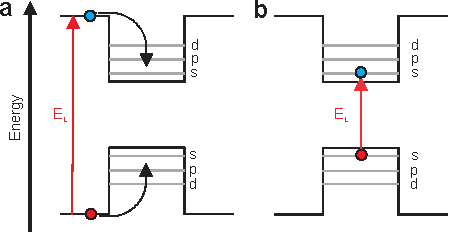
\includegraphics[width=0.7\linewidth]{figures/quantum-dot/optical-pumping-quantum-dot}
	\caption{Optical pumping of a QD by	(a) above-band excitation and (b) resonant excitation~\cite{huber_gaas_2019}}
	\label{fig:optical-pumping-quantum-dot}
\end{figure}
Due to dipole-selection rules, resonant population of the $\ket{XX}$ state requires a two-photon-absorption process.
Hereby, the energy of a femtosecond-pulse laser $E_p$ is tuned to exactly the half of the \ac{XX} energy with respect to the ground energy $E_{P}$, as sketched in figure~\ref{fig:qd-resonant}.
Because of coulomb interaction two times the \ac{X} energy with respect to the ground energy $2 \cdot E_X$ is not equals $E_{XX}$ but differs by the binding energy $E_B$.
The laser is therefore tuned to 
\begin{equation}
E_P = E_X - E_B / 2
\end{equation}
Empirically $E_B \approx \SI{3.78}{\milli \electronvolt}$ for \ac{GaAs} \acp{QD}.
Resonant two-photon absorption is a third-order non-linear effect which involves two photons and electrons at once.
It depends on the third-order-susceptibility $\chi^{(3)}$ of \ac{GaAs} and therefore requires relatively high laser power.

As this two-level system is driven in resonance its population exhibits Rabi oscillations.
The final population of the \ac{XX} can be described by
\begin{equation}
N_{XX} = \sin^2\left(\frac{\theta}{2}\right)
\end{equation}
with $\theta$ as the pulse area in relation to the Rabi oscillations. $\theta$ is not the area of the excitation pulse, but depends on it in a non-trivial way~\cite{stufler_two-photon_2006}.
Measured Rabi oscillations of \ac{X} and \ac{XX} are shown in figure~\ref{fig:rabi-oscillations}~\cite{reindl_phonon-assisted_2017}.
Theoretically, the curve should oscillate between occupancies $N/N_0$ of $0$ and $1$.
However, as a consequence of phonon damping the occupancy converges to a purely probabilistic value of $0.5$~\cite{forstner_phonon-assisted_2003}.
\begin{figure}[H]
	\centering
	\begin{subfigure}[b]{0.48\textwidth}
		\centering
		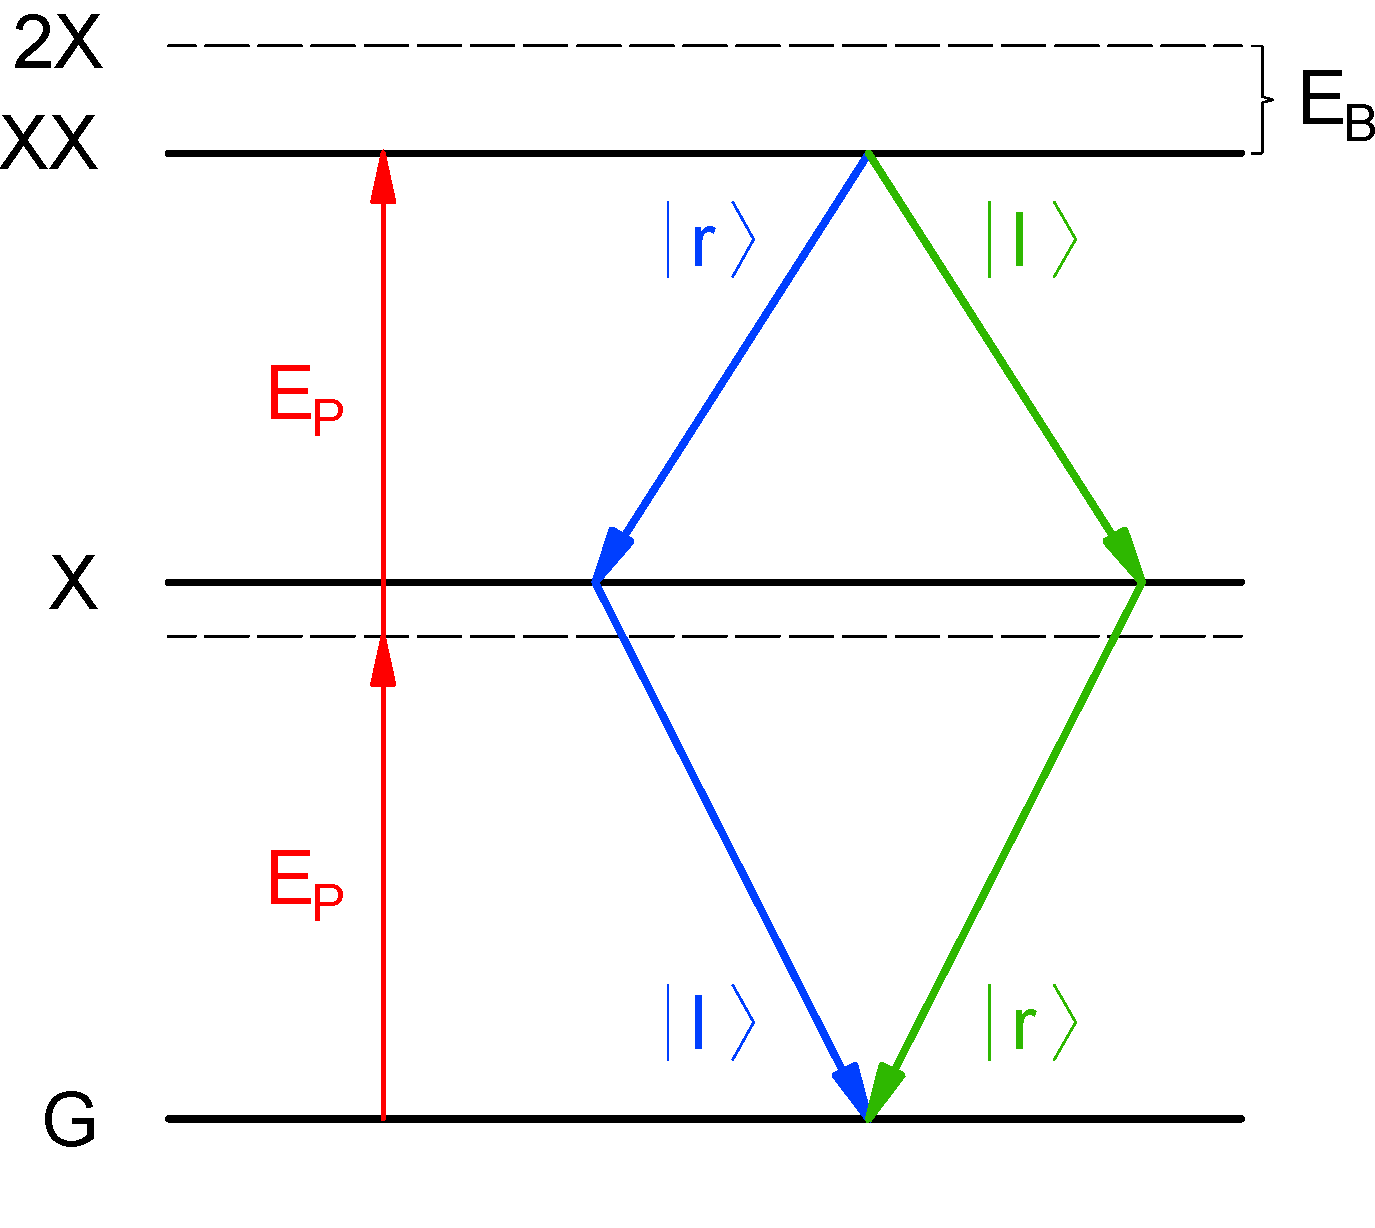
\includegraphics[width=0.95\textwidth]{figures/quantum-dot/QD_Resonant.pdf}
		\caption{Resonant two photon excitation of \ac{XX}.\\
			The laser is tuned to $E_P = E_{XX} / 2$.}
		\label{fig:qd-resonant}
	\end{subfigure}%
	~ % An dieser Stelle kann ein zusätzlicher Zwischenraum eingebunden werden: ~, \quad, \qquad, \hfill usw.
	% Eine leere Zeile erzwingt, dass die zweite Grafik darunter erscheint.
	\begin{subfigure}[b]{0.48\textwidth}
		\centering
		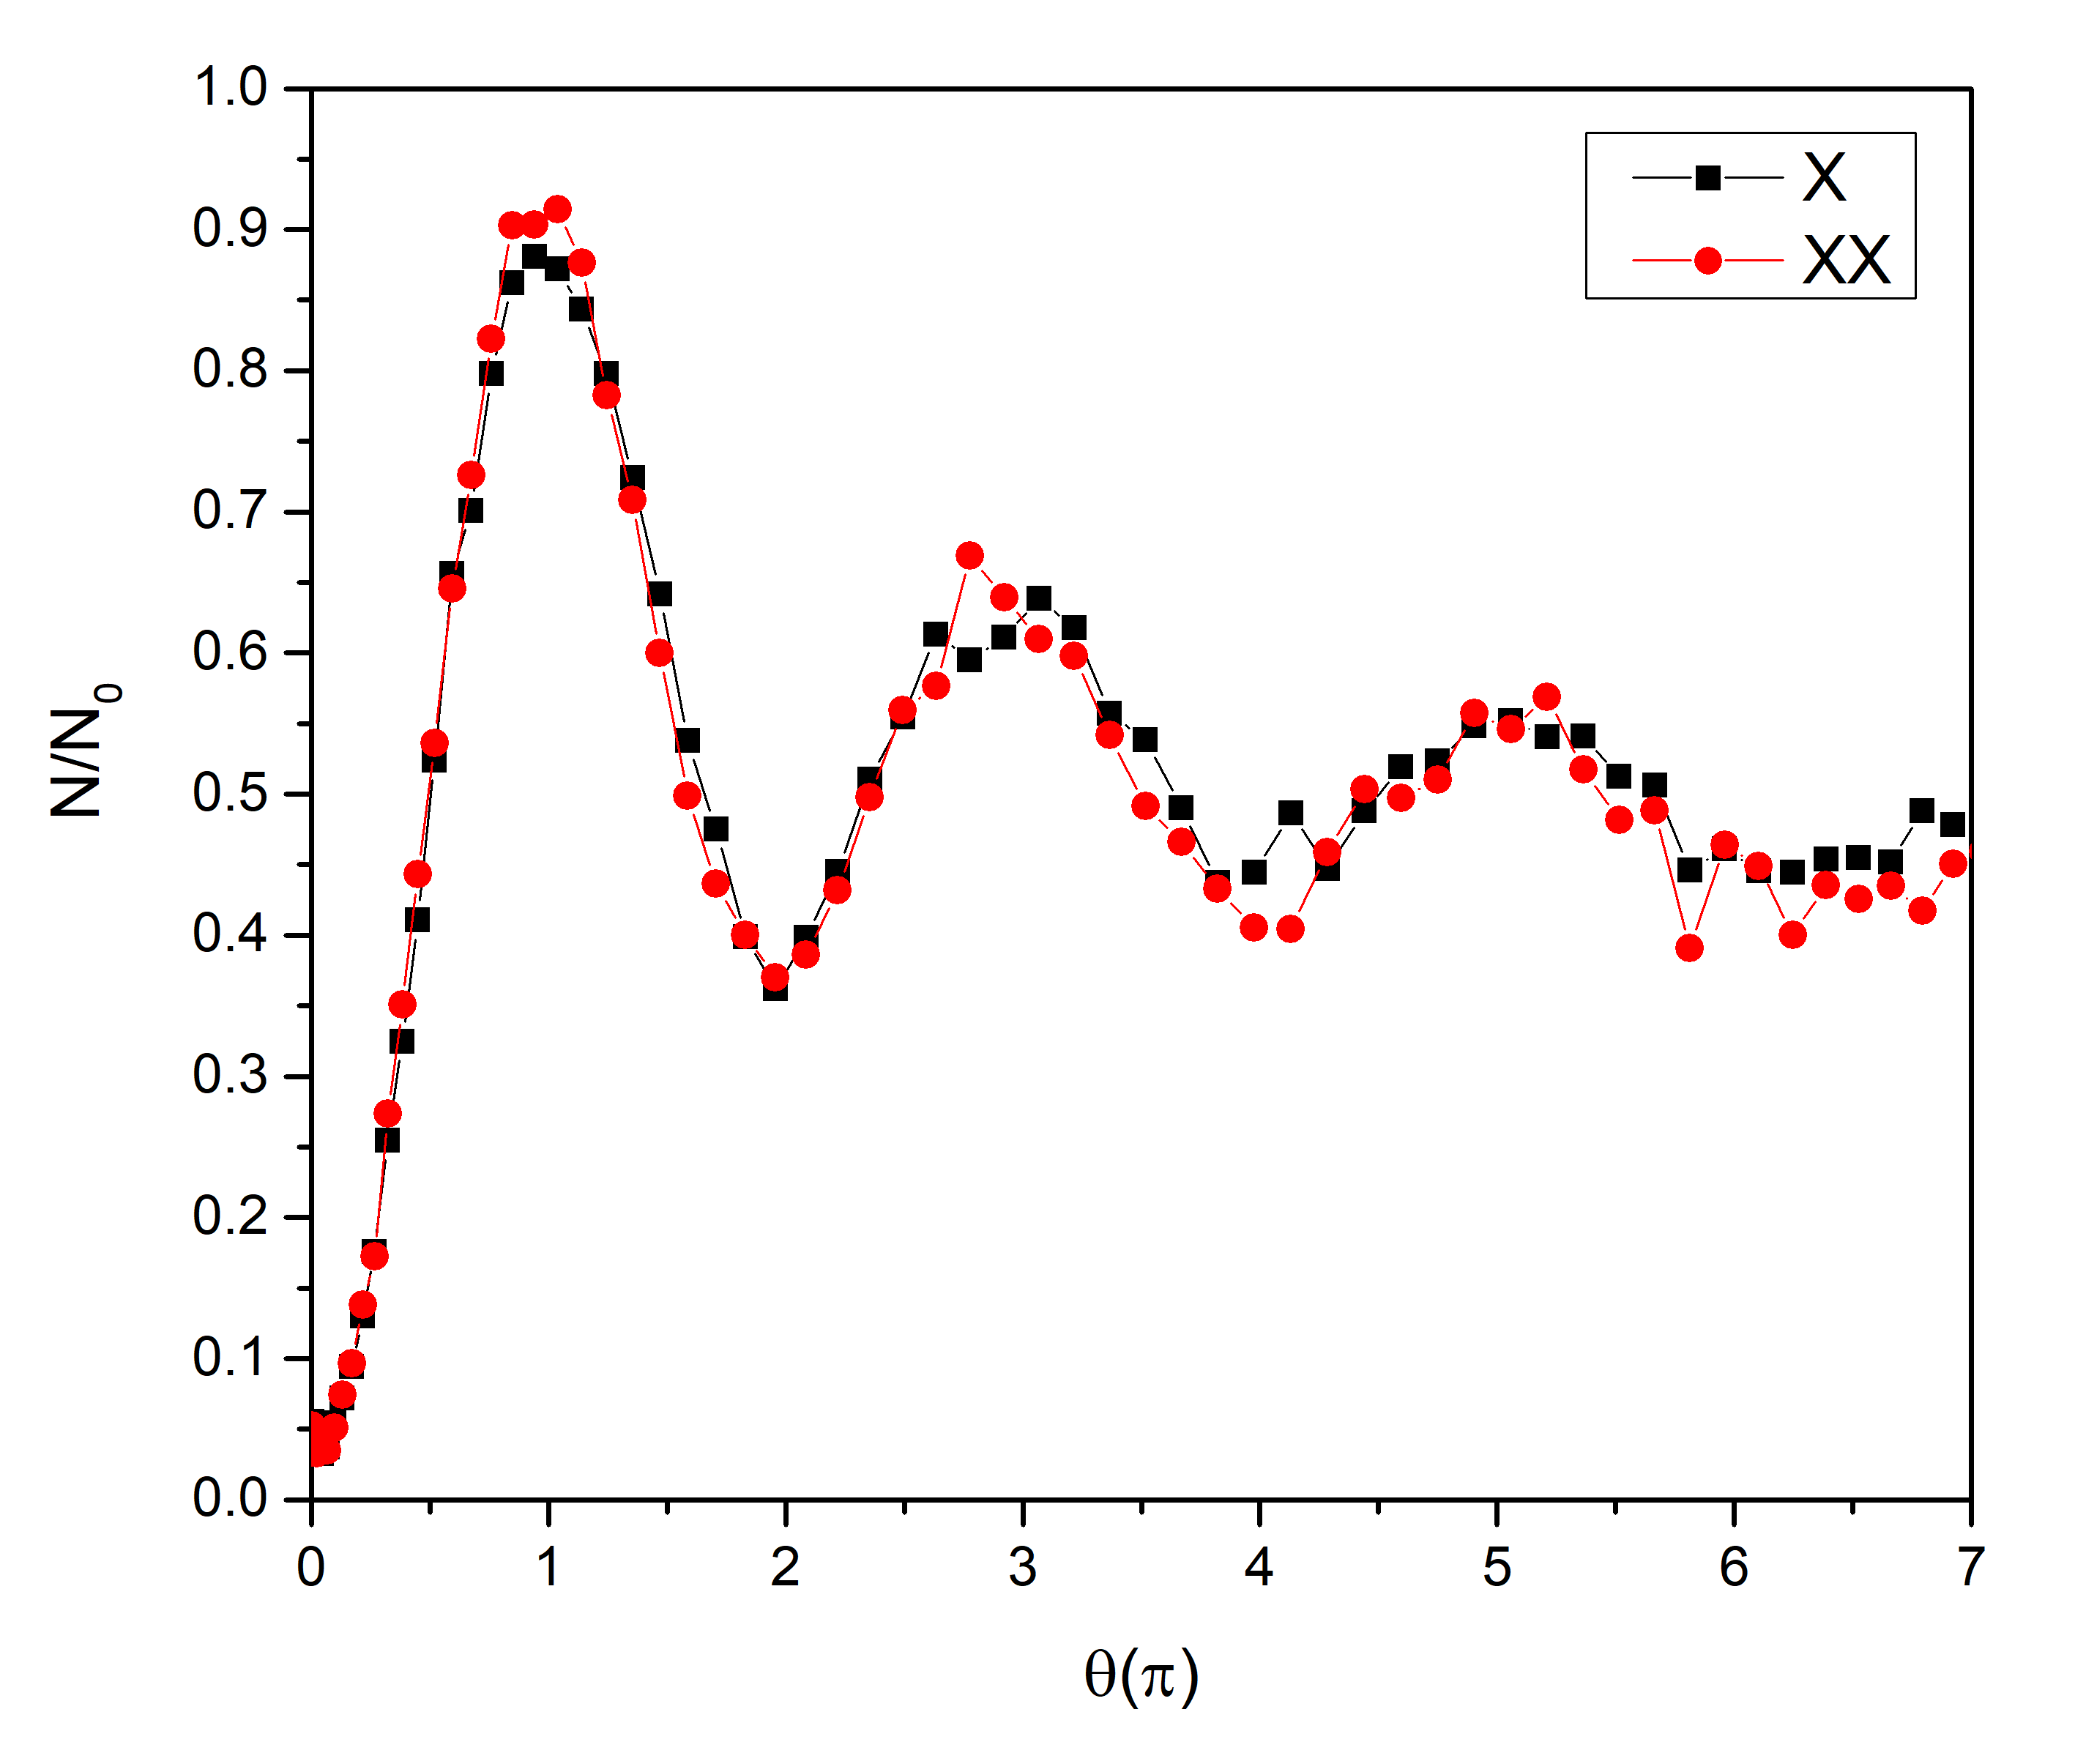
\includegraphics[width=\textwidth]{figures/quantum-dot/Rabi_Oscillations_rel.png}
		\caption{Rabi oscillations of \ac{X} and \ac{XX} as a function of the pulse area $\theta$.
				$N/N_0$ is the occupancy and $N_0$ the maximum population.}
		\label{fig:rabi-oscillations}
	\end{subfigure}
	\caption{Resonant two photon excitation~\cite{schimpf_towards_2017}}
	\label{fig:resonant-two-photon-excitation}
\end{figure}
\section{Single photon emission}
The XX-X cascade shown in figure~\ref{fig:qd-resonant} results in a single photon pair per emission cycle.
Single photons are necessary for quantum cryptography and quantum optics in general which motivates the following discussion of this topic based on the thesis of \textcite{huber_gaas_2019}.
The single photon purity of the $\ket{XX}$ to $\ket{X}$ and the $\ket{X}$ to $\ket{G}$ signals, respectively, can be determined by performing a \acf{HBT} experiment.
A \ac{HBT} setup is shown in figure~\ref{fig:hbt-fiber} and it allows to measure the second-order correlation function, which is defined as
\begin{equation}
g^{(2)} = \frac{\langle I(t) I(t+\tau)\rangle}{\langle I(t) \rangle \langle I(t+\tau)\rangle}
\end{equation}
with $I(t)$ as the light intensity and $\tau$ as the time delay. When a single photon enters the input of the \ac{BS} it can only be measured at one output, but never at both simultaneously.
Assuming a perfect single photon emitter, a coincidence measurement between APD1 and APD2 will result in $g^{(2)}(\tau) = 0$ at zero time delay.
Subsequently, side peaks are expected which are correlated to the repetition rate $R$ of the laser by $\tau_s=z/R$ with $z\in \mathbb{Z}\backslash \{0\}$.
The single photon purity can then be defined as
\begin{equation}
\kappa(b) = \frac{A_0(b)}{A_s(b)}
\end{equation}
with $A_0$ as the area under $g^{(2)}(\tau)$ around $\tau=0$ and $A_s$ as the average area under the side peaks at $\tau_s$.
The time bin $b$ has to be chosen so that it includes a full side peak.
If $b$ would be chosen too small it would falsely increase $\kappa$, if chosen too high it includes unnecessary much noise.

\begin{figure}[H]
	\centering
	\begin{subfigure}[b]{0.48\textwidth}
		\centering
		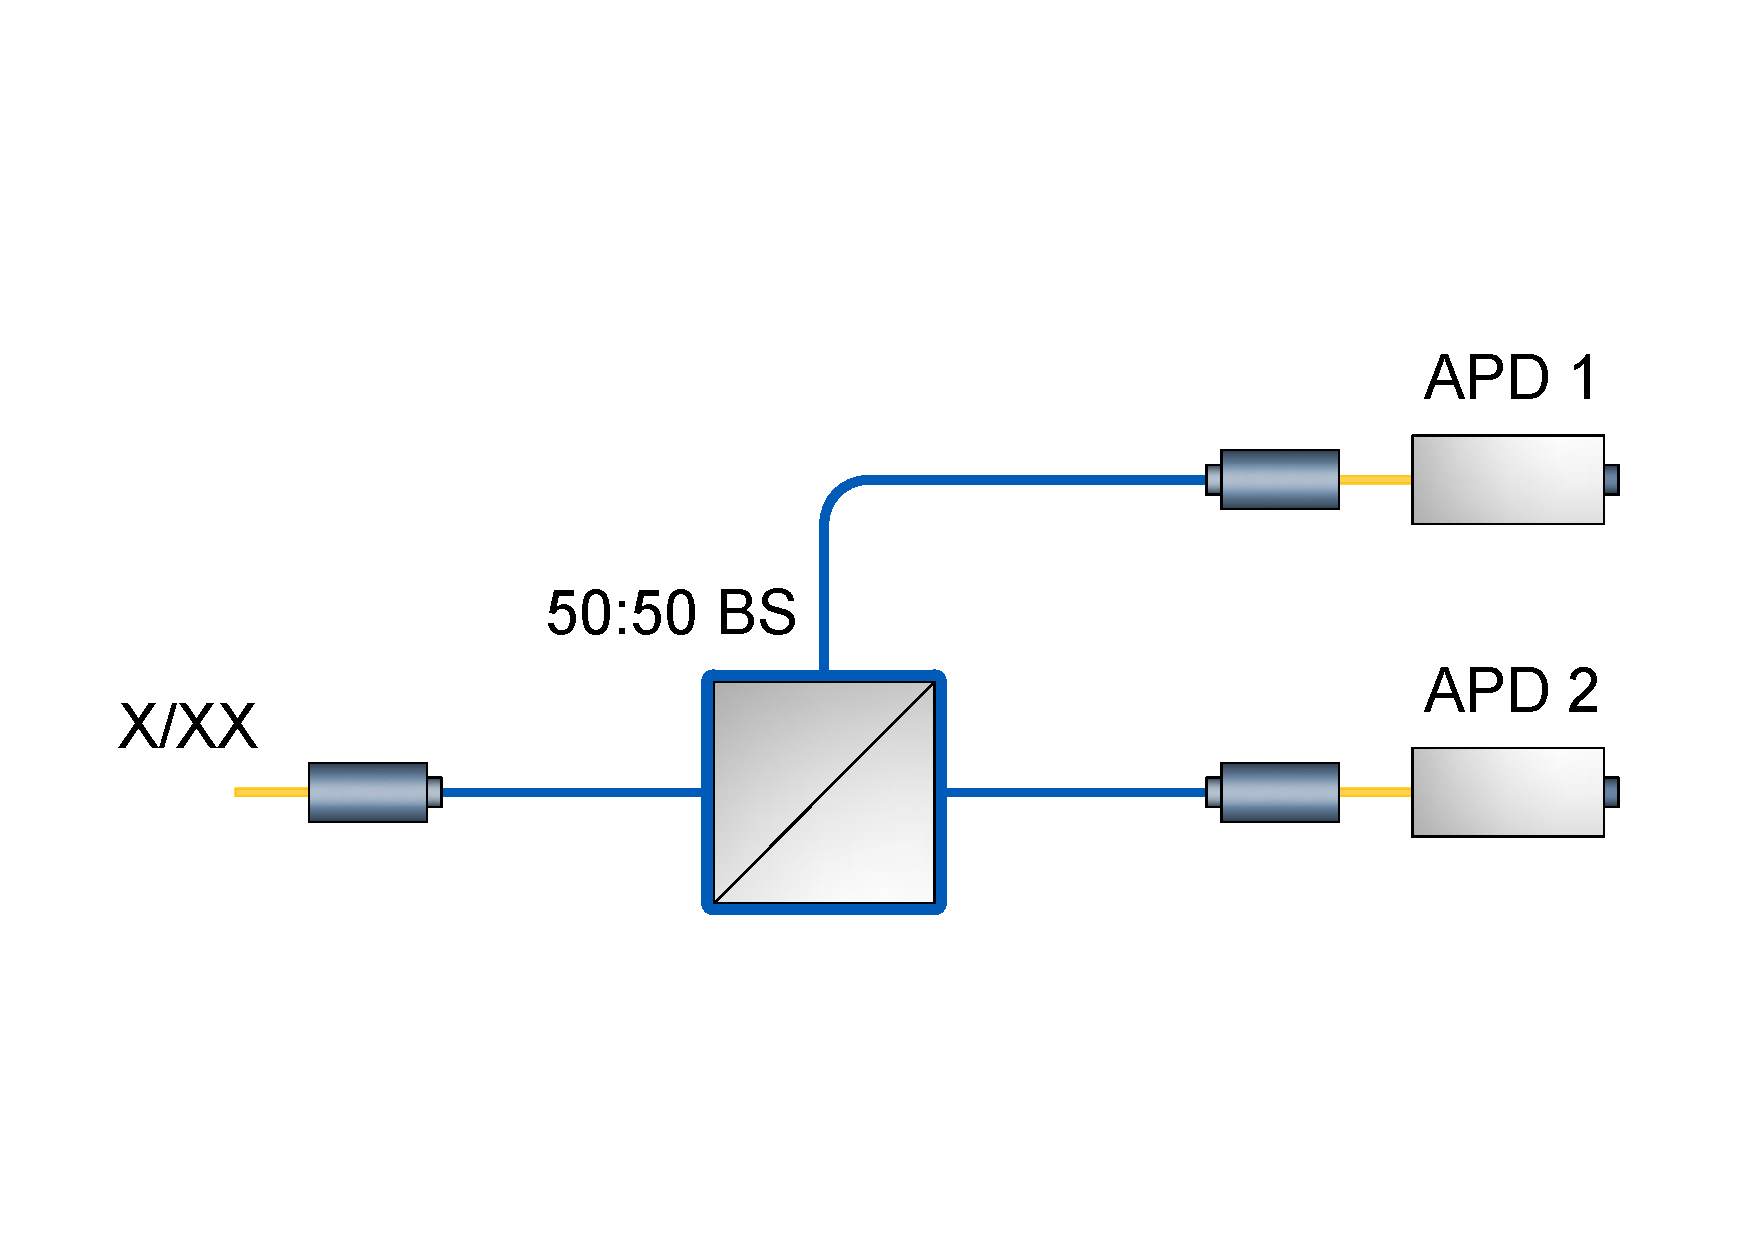
\includegraphics[width=0.95\textwidth]{figures/quantum-dot/HBT_Fiber.pdf}
		\caption{Setup to measure to measure the Hanbury-Brown-Twiss effect.}
		\label{fig:hbt-fiber}
	\end{subfigure}%
	~ % An dieser Stelle kann ein zusätzlicher Zwischenraum eingebunden werden: ~, \quad, \qquad, \hfill usw.
	% Eine leere Zeile erzwingt, dass die zweite Grafik darunter erscheint.
	\begin{subfigure}[b]{0.48\textwidth}
		\centering
		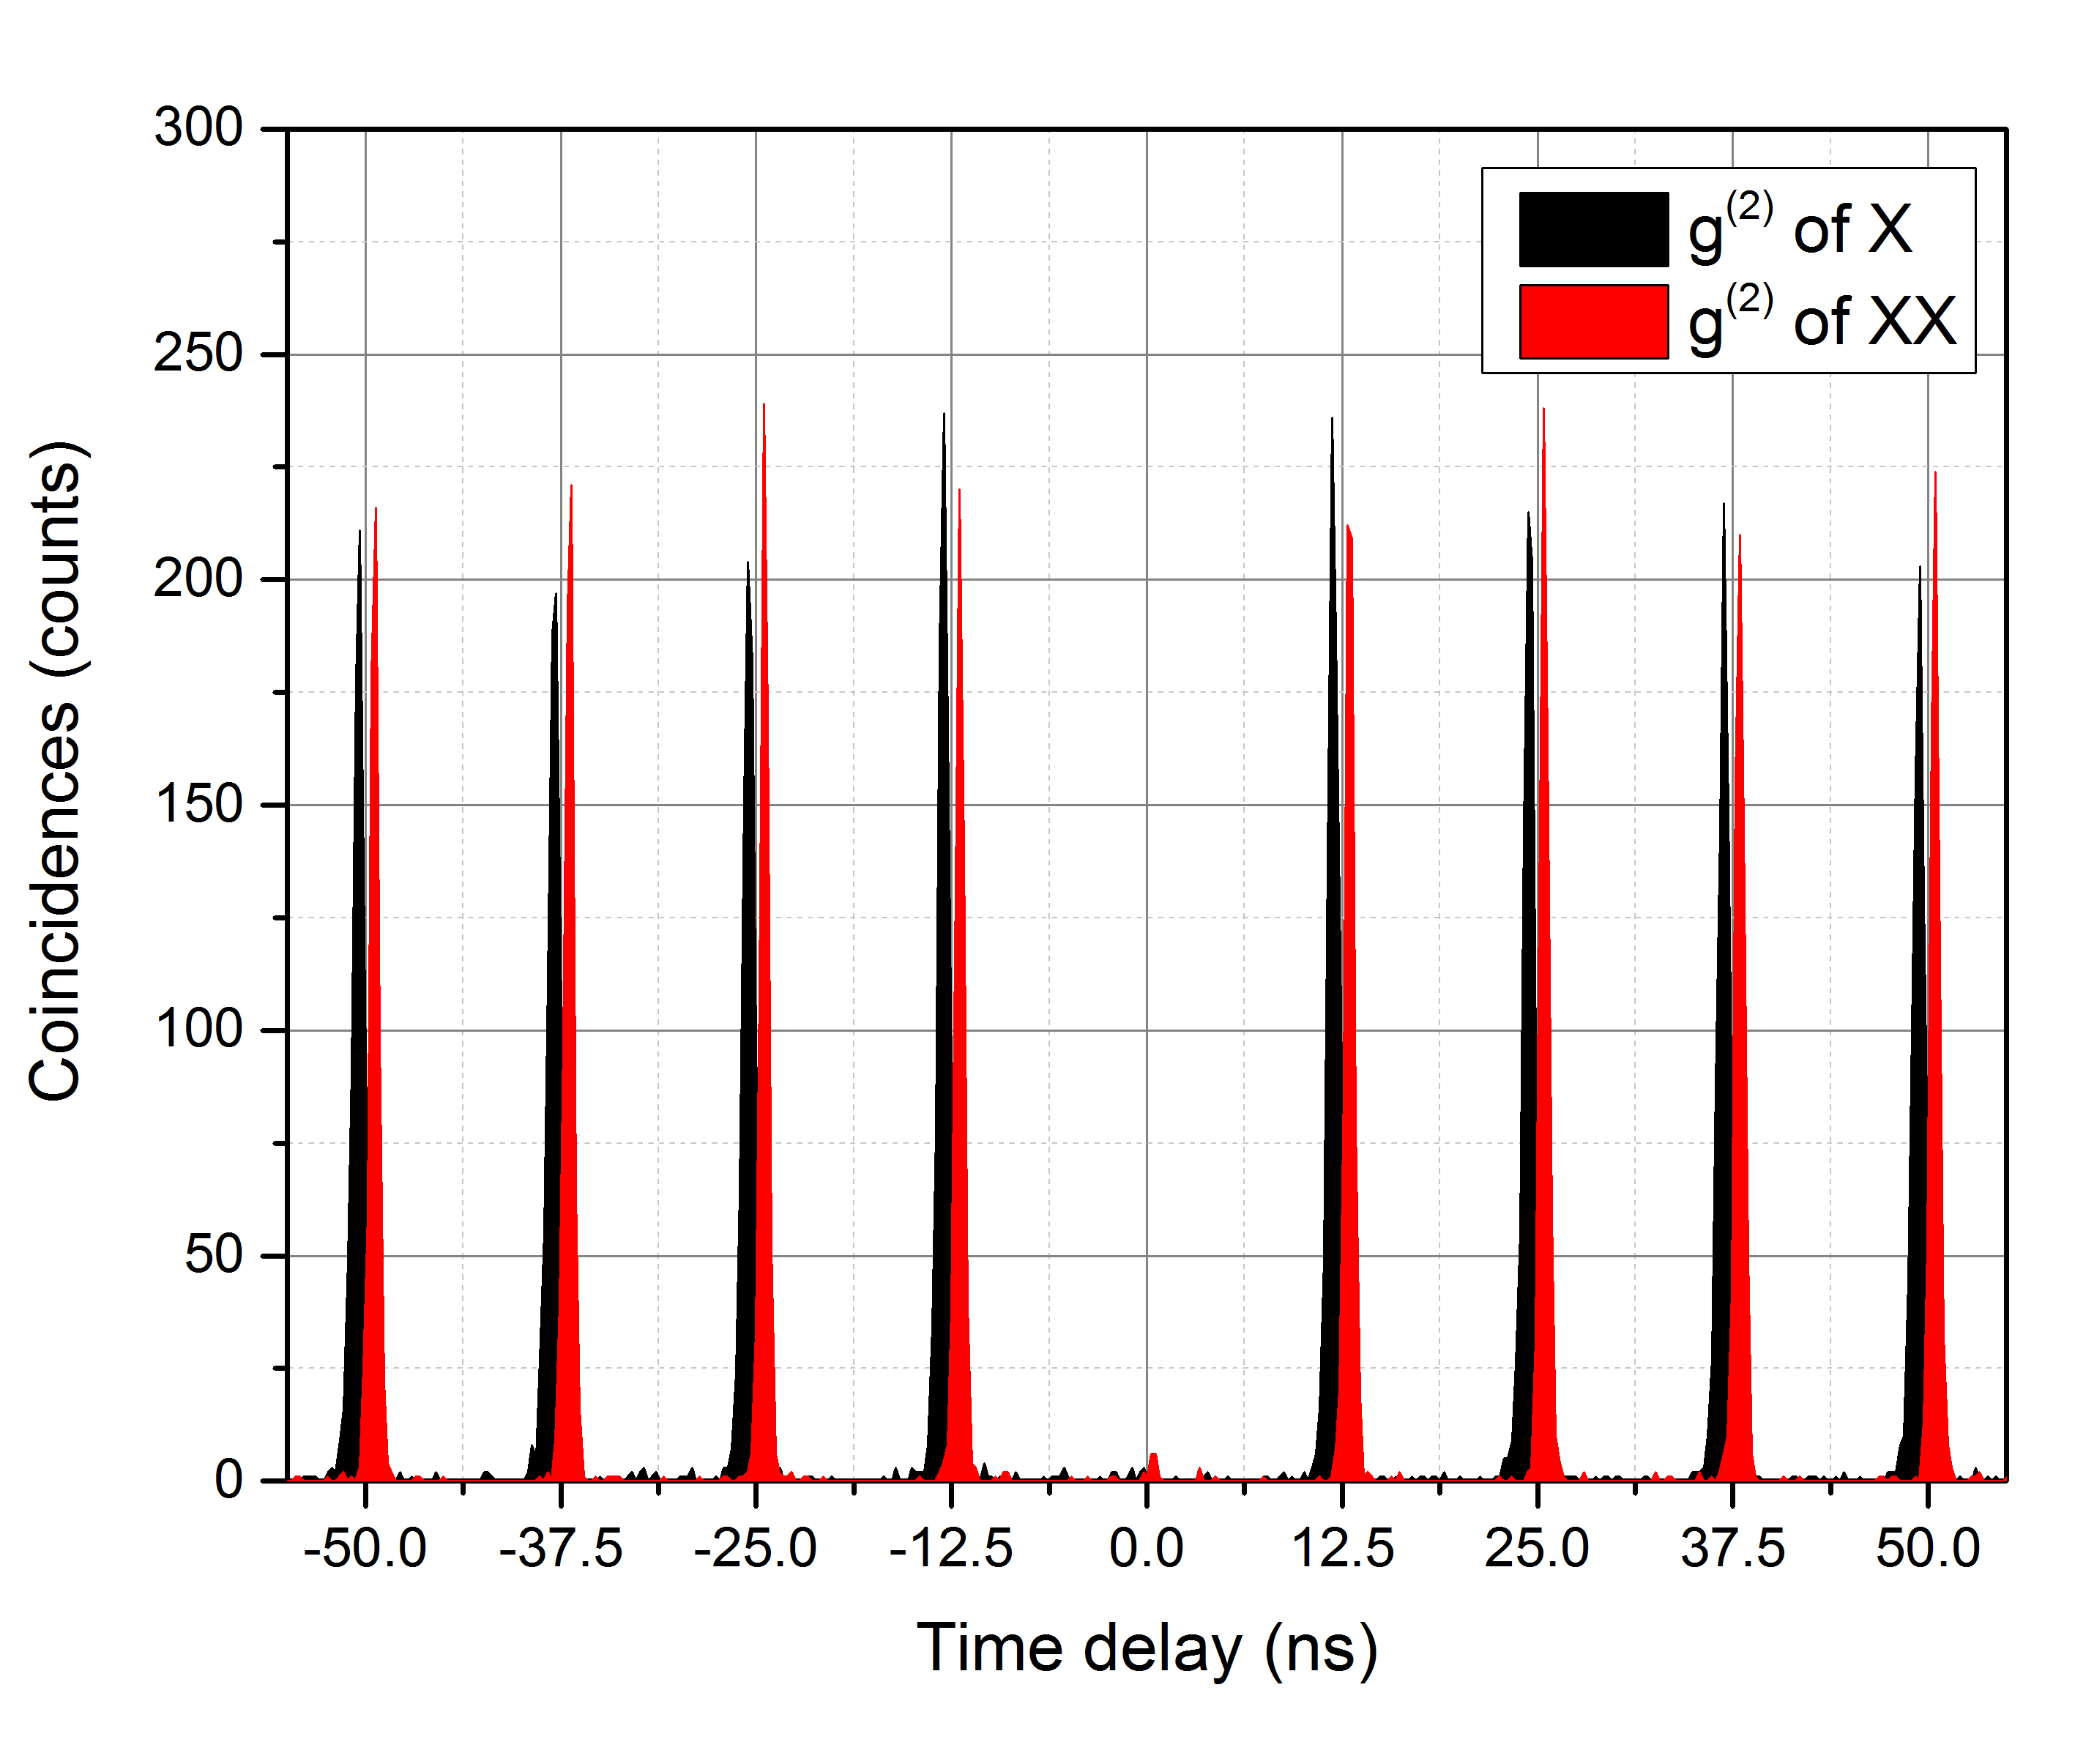
\includegraphics[width=\textwidth]{figures/quantum-dot/G2_X_XX.png}
		\caption{Second-order auto-correlation function $g^{(2)}$ of \ac{X} and \ac{XX}.}
		\label{fig:gs2-x-xx}
	\end{subfigure}
	\caption{Hanbury-Brown-Twiss \acs{HBT} experiment~\cite{schimpf_towards_2017}}
	\label{fig:hbt}
\end{figure}
  

